\documentclass[a4paper,11pt]{article}
\usepackage[T1]{fontenc}
\usepackage[utf8]{inputenc}
\usepackage[english]{babel}
\usepackage{lmodern}
\usepackage{color}
\usepackage{listings}
\usepackage{hyperref}
\usepackage[top=3cm, bottom=3cm, left=3cm, right=3cm]{geometry}
\usepackage{graphicx} 

\hypersetup{
    colorlinks,
    linkcolor=black,
    urlcolor=blue
}


\lstset{
	tabsize=4,
        basicstyle=\scriptsize,
        %upquote=true,
        aboveskip={1.5\baselineskip},
        columns=fixed,
        showstringspaces=false,
        extendedchars=true,
        breaklines=true,
        prebreak = \raisebox{0ex}[0ex][0ex]{\ensuremath{\hookleftarrow}},
	frame=single,
        showtabs=false,
        showspaces=false,
        showstringspaces=false,
        identifierstyle=\ttfamily,
        keywordstyle=\color[rgb]{0,0,1},
        commentstyle=\color[rgb]{0.133,0.545,0.133},
        stringstyle=\color[rgb]{0.627,0.126,0.941},
        framerule=0pt,
	language=Python
}





\title{Internationalization and localization with Limnoria~/~Supybot}
\author{Valentin "ProgVal" Lorentz}
\date{}

\begin{document}

\maketitle
\tableofcontents

\newpage

\part{Internationalizing your plugins}
  \section{About gettext}

    Gettext is a really powerful tool to internationalize software, and many
    other tools come with it, that's why I first wanted to use it.
    But, the problem was gettext need to have a single catalog for the whole
    software, but that is impossible for Supybot because of its modularity:
    each plugin needs to have its own catalog of translations.

    Then, I choosed to write my own internationalization tool, compatible with
    tools designed for gettext (such as PoEdit or pygettext), fully integrated
    with Limnoria.
    
    For plugins developpers, the syntax to use is nearly the same.
    
  \section{Importing the i18n module}
    
    i18n is the short version of "internationalization". It is also the name
    I gave to the module which handles internationalization and localization
    in Limnoria. All internationalized plugins need to import and use it.
    
    If you created your plugin with the modified version of
    supybot-plugin-create provided with Limnoria, your plugin already imports
    the i18n module. If you didn't use the modified tool, append this code
    after the imports, in \emph{plugin.py} and \emph{config.py}:
    \begin{lstlisting}[language=python]
      from supybot.i18n import PluginInternationalization
      from supybot.i18n import internationalizeDocstring
      _ = PluginInternationalization('<NAME OF YOUR PLUGIN>')
    \end{lstlisting}
    
    But this code has a problem: as you see, it requires the module
    \emph{supybot.i18n}, and this module exists only in Limnoria (at the
    moment).
    Then, I suggest you to use this code:
    \begin{lstlisting}[language=python]
      try:
          from supybot.i18n import PluginInternationalization
          from supybot.i18n import internationalizeDocstring
          _ = PluginInternationalization('<NAME OF YOUR PLUGIN>')
      except:
          _ = lambda x:x
          internationalizeDocstring = lambda x:x
    \end{lstlisting}
    As you can see, if the import fails, the functions are replaced by
    functions which takes an argument, and return it verbatim.
    Of course, the string won't be localized, but it is still better than
    an error.
  
  \section{It is time to internationalize!}
    \subsection{Internationalize the docstrings}
      As you probably noticed, Supybot uses the docstrings of the command as
      help. This help should be internationalized.
      
      To do that, the i18n module provides the function
      \emph{internationalizeDocstring}. I know this name is long, I have to
      use it for all commands I write for my plugins, but I think having an
      explicit name is more important than having a short name. Thanks to
      this long name, you know what it does: it internationalizes the
      docstrings!
      
      Actually, this function is a decorator. If you don't know what a
      decorator is, that is not important. You just have to add a line
      before every command, like that:
      \begin{lstlisting}[language=python]
        @internationalizeDocstring # <= This is the line
        def mycommand(self, irc, msg, args, arg1, arg2):
          """<argument 1> <argument 2>
          
          This command does that"""
          # The code of the command
        mycommand = wrap(mycommand, ['something', 'something'])
      \end{lstlisting}
      
      Additionally, you can also decorate the class:
      \begin{lstlisting}[language=python]
        @internationalizeDocstring # <= This is the line
        class MyPlugin:
          """My plugin does that."""
          # The code of the plugin
        
        Class = MyPlugin
      \end{lstlisting}
      
    \subsection{Internationalize the strings}
      There is two types of strings: those displayed on IRC (irc.reply(),
      irc.error(), ...), and those which are not (log.debug(), log.info(),
      ...).
      I consider the bot owner (the only one who can read the logs) should
      be able to understand English, so we translate only the string displayed
      on IRC. This shorten the painful work of translating.
      
      To internationalize a string, the syntax is the same as gettext, because
      it is a good syntax, but also because it allows us to use tools designed
      for gettext (as pygettext). If you never used gettext, you will like
      the easiness of this syntax:
      \begin{lstlisting}[language=python]
        irc.reply(_('This is an internationalized string.'))
      \end{lstlisting}
      Really easy, isn't it?
      
      Now, we have another problem: how to insert variables into the string?
      You probably want to use one of this lines:
      \begin{lstlisting}[language=python]
        irc.reply(_('There is ' + count + ' packages on this repository'))
        irc.reply(_('There is %i packages on this repository' % count))
      \end{lstlisting}
      But you are wrong: in the best case, you will get an error. In the
      worst, the string won't be localized.
      The good syntax is:
      \begin{lstlisting}[language=python]
        irc.reply(_('There is %i packages on this repository') % count)
      \end{lstlisting}
  
  \section{Generate the POT file}
    All internationalized plugins should come with a POT file, usually named
    \mbox{messages.pot}.
    If you already used gettext, you probably want to use the gettext command
    to generate this file, but you are wrong. Do you remember the docstrings
    needs to (and will) be localized, even if we did not \_()-ize them? But
    gettext picks out only \_()-ized strings, so, it is not the tool we need.
    
    Fortunatly, a such tool exists! It is called pygettext and should be
    installed with Python. Here is the command to use:
    \begin{lstlisting}[language=bash]
      pygettext --docstring config.py plugin.py
    \end{lstlisting}
    It will create a file called messages.pot, which is needed by the
    translators.

\newpage
\part{Localizing plugins into your language}
  \section{Understanding the file formats}
    The localization process deals with three file types
    \begin{description}
      \item[a .pot] -- Contains untranslated strings. Human
        readable, but doesn't need to be read
      \item[a .po per language] -- Also called "catalog". It is the
        translation of the strings. Human readable.
      \item[a .mo per .po] -- The compiled version of the .po. Not human
        readable.
    \end{description}
    As I said before, Limnoria uses my own implementation of gettext; and
    this implementation does not need the .mo files: it reads directly the
    .po (actually, at the moment I was writing the i18n module, I did not
    know .mo files exist ;) ).
      
  \section{The tools}
    I personnaly use PoEdit, because it does everything one could expect on
    a PO editor: create the PO from the POT, nice PO editor, and PO -> MO
    compiler (even if we do not need the last one).
    
    But, PoEdit is not \emph{the} universal tool, there is many other
    graphic tools or in the console. I will not cover this other tools
    here because I never tryed them, but there is probably nice documentation
    somewhere else, but the process is nearly the same.
    
  \section{The files architecture used by Limnoria for its translations}
    There is two kind of localization files: for the core itself, and for
    the plugins.
    
    \begin{description}
      \item{The core}: The localization files of the core are in the
        directory locale/, located at the root of the source. There is two
        files per language: a fr.po and fr.py (fr is of course the language
        representation).
        
        The first one is  easy to understand and translate, it is a big
        classic PO file, translatable with PoEdit.
        
        fr.py is slightly more tricky: it contains additional Python code used
        to "say" how to do some stuff related to the language, such as
        pluralization. If you want to localize it, you need to be a Python
        programmer (actually, a beginner should be able to do it, it is easy).
        
      \item{The plugins}: All plugins should have a locale/ directory (create
        it if it does not exist), containing the PO files.
    \end{description}
    
  \section{Generate the PO file}
    \begin{figure}
      \begin{center}
        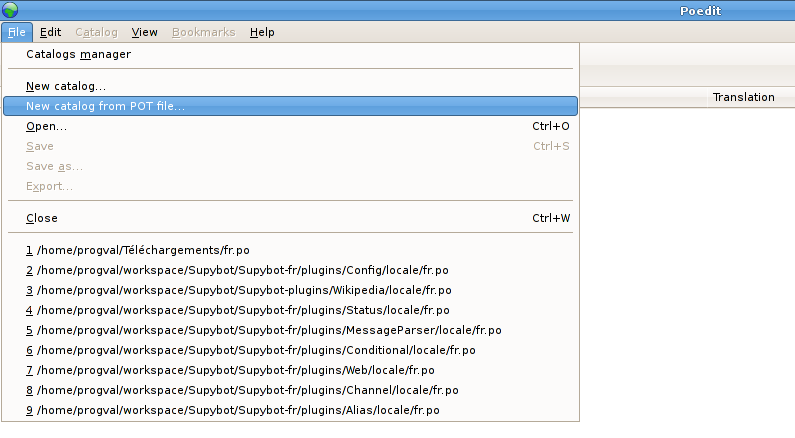
\includegraphics[scale=0.5]{pictures/new_catalog_from_POT_file.png}
        \caption{Creating a catalog from a .pot file}
        \label{fig:creating_a_catalog}
      \end{center}
    \end{figure}
    If you are editing an existing translation, skip this step.
    
    For Limnoria core, the POT is in the locale/ directory. For the plugins,
    it is in the directory of the plugin. (It is easy to remember, isn't it?)
    PoEdit allows you to create a catalog from the POT easily, from the File
    menu, as in figure~\ref{fig:creating_a_catalog}.
    Now you created the PO file, save it as
    \mbox{plugins/<plugin name>/locale/<language code>.po} if it is for a
    plugin or as \mbox{locale/<language code>.po} if it is for the core.
  
  \section{Translate the PO file}
    \begin{figure}
      \begin{center}
        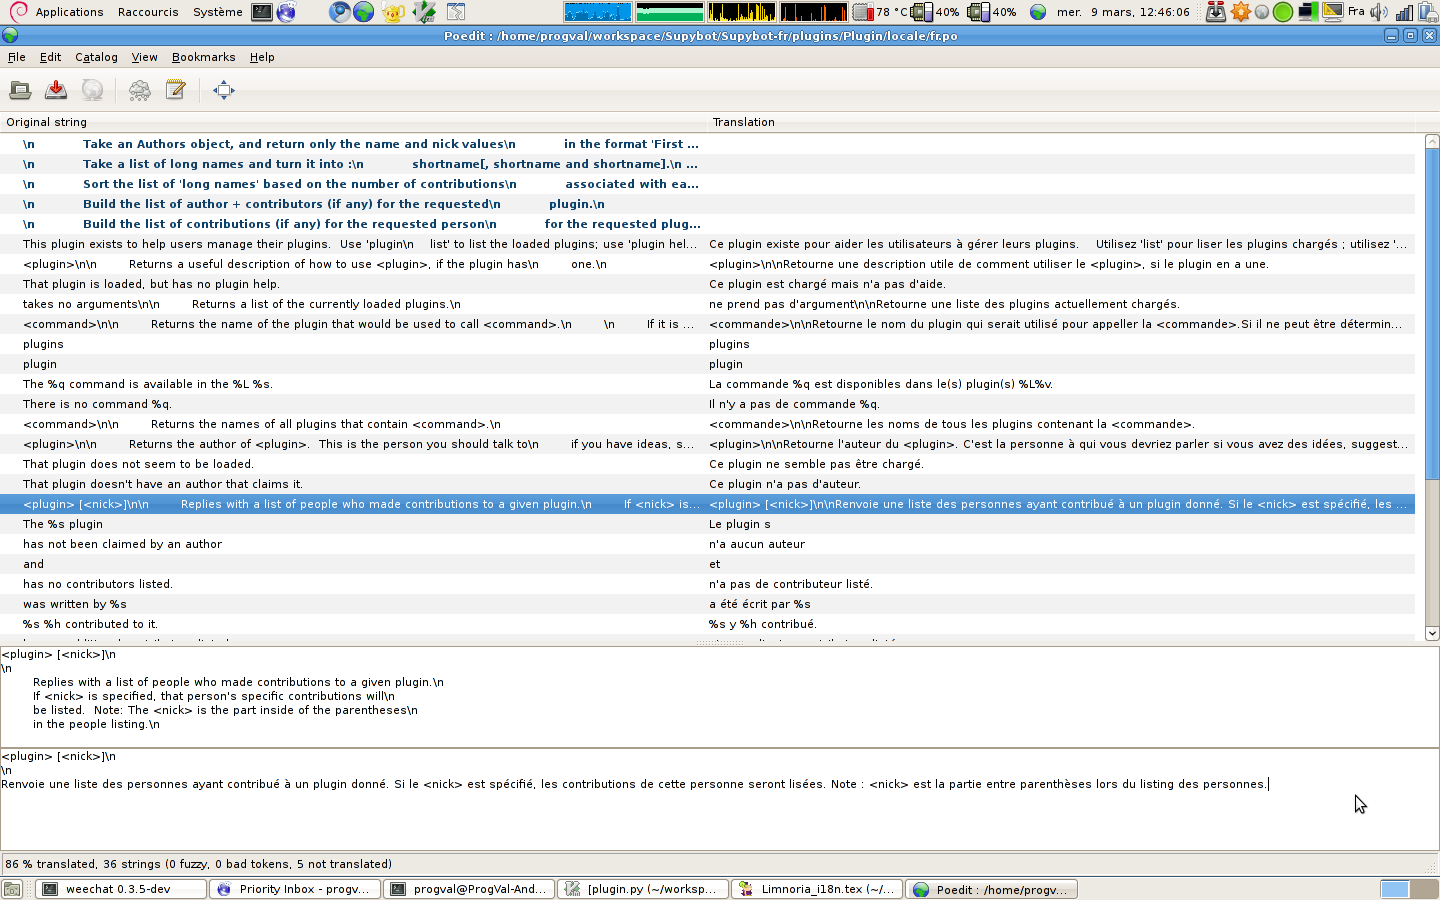
\includegraphics[scale=0.25]{pictures/translate_the_strings.png}
        \caption{Translating the strings}
        \label{fig:translating_the_strings}
      \end{center}
    \end{figure}
    Now, the most important step: translating the plugin/bot. Open it with
    PoEdit or with your favorite PO editor, and translate it, as in
    figure~\ref{fig:translating_the_strings}.
    
    There is two things you have to keep in mind:
    \begin{itemize}
      \item In the untranslated string, there is many \textbackslash{}n and 
        line break. You can ignore them safely, they are useless...
      \item ... but you need to have two \textbackslash{}n after the syntax
        of commands. That is important, Limnoria uses them to detect what is
        the syntax and what is the real help (when displayed on IRC, the
        syntax is bold).
    \end{itemize}
    
    


    
\clearpage
\newpage
\part*{About}
  \section*{More informations}
    If you need more informations, you can contact me on \mbox{\#supybot} or
    \mbox{\#supybot-fr} on Freenode IRC Network.
    You can also contact me by email, I should answer in less than a week.
  
  \section*{Getting this document}
    Of source, this is a libre document. You can access source code at
    \href{https://github.com/ProgVal/Supybot-docs}{GitHub}.
  
  \section*{Licencing}
    This work is licensed under a Creative Commons Attribution 3.0 Unported License.
    \paragraph{You are free:}
      \begin{description}
        \item[toShare] -- to copy, distribute, and transmit the work
        \item[toRemix] -- to adapt the work
      \end{description}

    \paragraph{Under the fellowing condition:}
      \begin{description}
        \item[Attribution] -- You must attribute the work in the
manner specified by the author or licensor (but not in any way that suggests
that they endorse you or your use of the work). 
        
      \end{description}


\end{document}
